\documentclass[tikz,border=10pt]{standalone}
\usepackage{tikz}
\usetikzlibrary{patterns, arrows.meta, positioning, calc}

\begin{document}
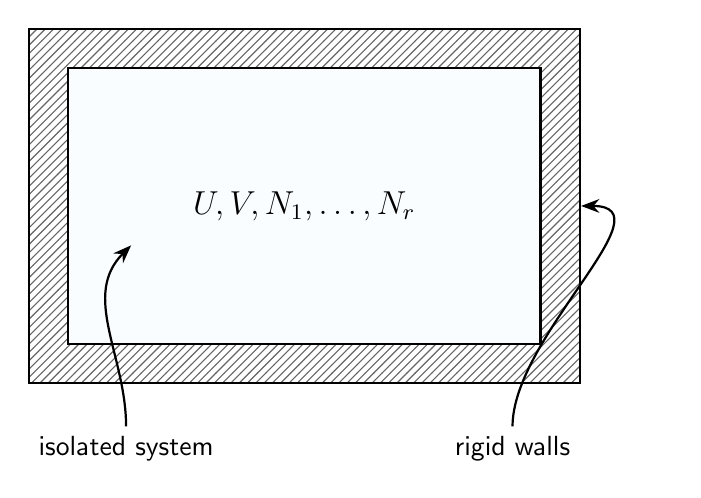
\begin{tikzpicture}
    % --- Style Definitions ---
    \tikzset{
        wall style/.style={
            draw=black, 
            thick, 
            pattern=north east lines, 
            pattern color=black!60
        },
        system style/.style={
            draw=black, 
            thick, 
            fill=cyan!2, 
            minimum width=6cm, 
            minimum height=3.5cm,
            outer sep=0pt
        },
        label text/.style={
            font=\sffamily, 
            color=black
        },
        annotation arrow/.style={
            ->, 
            >=Stealth, 
            thick, 
            black
        }
    }

    % --- 1. Draw the Walls (Outer Box) ---
    \node[
        wall style, 
        minimum width=7cm, 
        minimum height=4.5cm
    ] (outer) at (0,0) {};

    % --- 2. Draw the System (Inner Box) ---
    \node[system style] (inner) at (0,0) {};

    % --- 3. System Variables ---
    \node[font=\large] at (0,0) {$U, V, N_1, \dots, N_r$};

    % --- 4. Annotations ---

    % Left Annotation: Isolated System
    \node[label text, anchor=north west] (lbl_iso) at (-3.5, -2.8) {isolated system};
    
    % ADJUSTMENT HERE: 
    % Changed target from center-ish to (-2.2, -0.5)
    % This points to the empty space on the left side
    \draw[annotation arrow] (lbl_iso.north) to[out=90, in=225] (-2.2, -0.5);

    % Right Annotation: Rigid Walls
    \node[label text, anchor=north east] (lbl_wall) at (3.5, -2.8) {rigid walls};
    \draw[annotation arrow] (lbl_wall.north) to[out=90, in=0] (outer.east);

\end{tikzpicture}
\end{document}